\documentclass[10pt, letterpaper]{article}

% Packages:
\usepackage[
    ignoreheadfoot, % set margins without considering header and footer
    top=2 cm, % seperation between body and page edge from the top
    bottom=2 cm, % seperation between body and page edge from the bottom
    left=2 cm, % seperation between body and page edge from the left
    right=2 cm, % seperation between body and page edge from the right
    footskip=1.0 cm, % seperation between body and footer
    % showframe % for debugging
]{geometry} % for adjusting page geometry
\usepackage{titlesec} % for customizing section titles
\usepackage{tabularx} % for making tables with fixed width columns
\usepackage{array} % tabularx requires this
\usepackage[dvipsnames]{xcolor} % for coloring text
\definecolor{primaryColor}{RGB}{0, 79, 144} % define primary color
\usepackage{enumitem} % for customizing lists
\usepackage{fontawesome5} % for using iconsac
\usepackage{amsmath} % for math
\usepackage{graphicx} % for the profile photo
\usepackage[
    pdftitle={VINH-KHUONG TRUONG's CV},
    pdfauthor={VINH-KHUONG TRUONG},
    pdfcreator={LaTeX with RenderCV},
    colorlinks=true,
    urlcolor=primaryColor
]{hyperref} % for links, metadata and bookmarks
\usepackage[pscoord]{eso-pic} % for floating text on the page
\usepackage{calc} % for calculating lengths
\usepackage{bookmark} % for bookmarks
\usepackage{lastpage} % for getting the total number of pages
\usepackage{changepage} % for one column entries (adjustwidth environment)
\usepackage{paracol} % for two and three column entries
\usepackage{ifthen} % for conditional statements
\usepackage{needspace} % for avoiding page brake right after the section title
\usepackage{iftex} % check if engine is pdflatex, xetex or luatex

% Ensure that generate pdf is machine readable/ATS parsable:
\ifPDFTeX
    \input{glyphtounicode}
    \pdfgentounicode=1
    % \usepackage[T1]{fontenc} % this breaks sb2nov
    \usepackage[utf8]{inputenc}
    \usepackage{lmodern}
\fi



% Some settings:
\AtBeginEnvironment{adjustwidth}{\partopsep0pt} % remove space before adjustwidth environment
\pagestyle{empty} % no header or footer
\setcounter{secnumdepth}{0} % no section numbering
\setlength{\parindent}{0pt} % no indentation
\setlength{\topskip}{0pt} % no top skip
\setlength{\columnsep}{0cm} % set column seperation
\makeatletter
\let\ps@customFooterStyle\ps@plain % Copy the plain style to customFooterStyle
\patchcmd{\ps@customFooterStyle}{\thepage}{
    \color{gray}\textit{\small VINH-KHUONG TRUONG - Page \thepage{} of \pageref*{LastPage}}
}{}{} % replace number by desired string
\makeatother
\pagestyle{customFooterStyle}

\titleformat{\section}{\needspace{4\baselineskip}\bfseries\large}{}{0pt}{}[\vspace{1pt}\titlerule]

\titlespacing{\section}{
    % left space:
    -1pt
}{
    % top space:
    0.3 cm
}{
    % bottom space:
    0.2 cm
} % section title spacing

\renewcommand\labelitemi{$\circ$} % custom bullet points
\newenvironment{highlights}{
    \begin{itemize}[
        topsep=0.10 cm,
        parsep=0.10 cm,
        partopsep=0pt,
        itemsep=0pt,
        leftmargin=0.4 cm + 10pt  % Standard left margin for highlights
    ]
}{
    \end{itemize}
} % new environment for highlights

\newenvironment{highlightsforbulletentries}{
    \begin{itemize}[
        topsep=0.10 cm,
        parsep=0.10 cm,
        partopsep=0pt,
        itemsep=0pt,
        leftmargin=10pt
    ]
}{
    \end{itemize}
} % new environment for highlights for bullet entries


\newenvironment{onecolentry}{
    \begin{adjustwidth}{
        0.2 cm + 0.00001 cm
    }{
        0.2 cm + 0.00001 cm
    }
}{
    \end{adjustwidth}
} % new environment for one column entries

\newenvironment{twocolentry}[2][]{
    \onecolentry
    \def\secondColumn{#2}
    \setcolumnwidth{\fill, 4.5 cm}
    \begin{paracol}{2}
}{
    \switchcolumn \raggedleft \secondColumn
    \end{paracol}
    \endonecolentry
} % new environment for two column entries

% HEADER ENVIRONMENT DEFINITION (Restored closer to original)
\newenvironment{header}{
    \setlength{\topsep}{0pt}\par\kern\topsep\centering\linespread{1.5} % Original linespread
}{
    \par\kern\topsep
} % new environment for the header



% save the original href command in a new command:
\let\hrefWithoutArrow\href

% new command for external links:
\renewcommand{\href}[2]{\hrefWithoutArrow{#1}{\ifthenelse{\equal{#2}{}}{ }{#2 }\raisebox{.15ex}{\footnotesize \faExternalLink*}}}



\begin{document}
\pagestyle{empty}

\newcommand{\cvname}{VINH-KHUONG TRUONG}
\newcommand{\AND}{\unskip
    \cleaders\copy\ANDbox\hskip\wd\ANDbox
    \ignorespaces
}
\newsavebox\ANDbox
\sbox\ANDbox{}

% Name is provided by the including file (main.tex / main_vi.tex / cover letters)
% so the English and Vietnamese builds can share this contact block.
\providecommand{\cvname}{VINH-KHUONG TRUONG}

% Contact block, reused with and without the profile photo
\newcommand{\headercontent}{%
    \begin{header}
        \textbf{\fontsize{24 pt}{24 pt}\selectfont \cvname}
        \vspace{0.3cm}

        \normalsize
        \mbox{{\color{black}\footnotesize\faPhone*}\hspace*{0.13cm}0867084729}%
        \kern 0.25cm \AND \kern 0.25cm
        \mbox{{\color{black}\footnotesize\faEnvelope[regular]}\hspace*{0.13cm}\hrefWithoutArrow{mailto:trvinhkhuong@gmail.com}{trvinhkhuong@gmail.com}}%
        \kern 0.25cm \AND \kern 0.25cm
        \mbox{{\color{black}\footnotesize\faGithub}\hspace*{0.13cm}\hrefWithoutArrow{https://github.com/truongvinhkhuong}{github.com/truongvinhkhuong}}%
    \end{header}
}

% Drop an `image.jpg` into the repository root to show a profile photo.
% Without it the header simply renders full width.
\IfFileExists{image.jpg}{%
    \noindent
    \begin{minipage}[c]{0.78\textwidth}
        \headercontent
    \end{minipage}\hfill
    \begin{minipage}[c]{0.2\textwidth}
        \raggedleft
        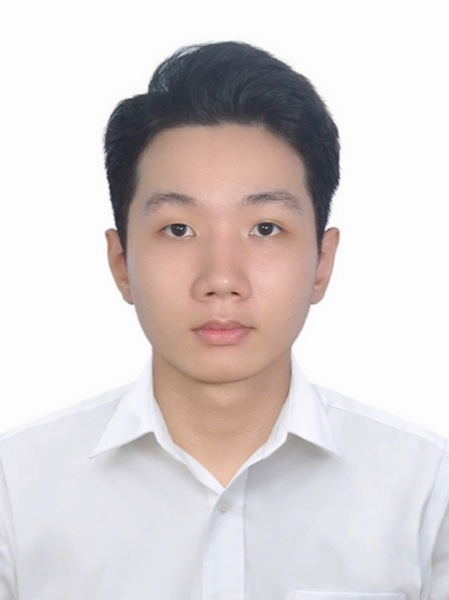
\includegraphics[width=2.5cm,height=3.5cm,keepaspectratio]{image.jpg}
    \end{minipage}
}{%
    \headercontent
}

\vspace{0.3 cm}


\vspace{0.5cm}

\begin{onecolentry}

Dear Hiring Manager,

\vspace{0.2cm}

I am writing to express my interest in the open software engineering position at your organization. As a Full-stack Developer with two years of experience building commerce and enterprise platforms end-to-end --- React/Next.js frontends, Node.js/NestJS backends, PostgreSQL data models, CI/CD and production operations --- I am confident I can contribute meaningfully to your team from day one.

\vspace{0.2cm}

In my current role at \textbf{Tierra Diamond}, a luxury diamond jewelry brand, I architected and built the company's commerce and customer platform from scratch as its core engineer. I built a \textbf{Zalo Mini App} with 60+ screens on React and TanStack Query, backed by a NestJS API on Drizzle/PostgreSQL, and designed sync pipelines that bring 116K+ customers and 77K+ order lines from the data warehouse and BEONE ERP into a Postgres read-model with validation gates and PII hashing at ingest. On the order side, I implemented a deposit lifecycle on \textbf{Medusa v2} with a transactional outbox, idempotency keys and RabbitMQ events, and set up GitHub Actions CI/CD with migration checks, Trivy scans and end-to-end OpenTelemetry tracing.

\vspace{0.2cm}

Before that, at \textbf{Truong Dinh Holdings}, I supported a phased migration from Bravo ERP to Odoo Community, built and deployed \textbf{toanthang.vn} on Next.js, NestJS and Payload CMS, and developed a \textbf{RAG chatbot} (FastAPI, LlamaIndex, Qdrant). As \textbf{Founding Engineer at UMIC (umic.ai)}, I architected a multi-tenant AI marketing SaaS from scratch, including a multi-agent content planner on LangGraph with real-time SSE streaming.

\vspace{0.2cm}

Earlier roles rounded out that foundation: automation engineering with n8n and Python at \textbf{BBI}, full-stack development on Python/Flask and Vue.js at \textbf{VNGroup Tourist}, and teaching programming at \textbf{MindX Technology School}, where reviewing student code sharpened how I communicate technical decisions.

\vspace{0.2cm}

\textbf{What I bring:}

\vspace{0.1cm}

\begin{highlights}
    \item \textbf{Full-stack Development:} React\slash Next.js, TypeScript, Node.js\slash NestJS, Medusa v2, FastAPI, PostgreSQL, Redis
    \item \textbf{Reliable Systems:} event-driven design with RabbitMQ, transactional outbox, idempotency, ERP and data-warehouse integration
    \item \textbf{DevOps \& Quality:} Docker, GitHub Actions CI/CD, Trivy, OpenTelemetry, Vitest, Jest, Cypress, SonarQube
    \item \textbf{Product Ownership:} taking features from requirement to production, from greenfield platforms to ERP migration
\end{highlights}

\vspace{0.2cm}

I enjoy work where engineering meets real business impact --- turning messy workflows into systems people actually rely on. I would welcome the opportunity to discuss how my background fits your team's needs.

\vspace{0.4cm}

Best regards,\\
\textbf{Vinh-Khuong Truong}

\end{onecolentry}

\end{document}
